\section{Enabling General Root Cause Analysis}
\label{sec:general}

In this section we discuss a general framework for root cause analysis,
challenges, and how we propose to overcome those challenges.

\subsection{Generic Root Cause Analysis}

\begin{figure}[!htbp]
\centering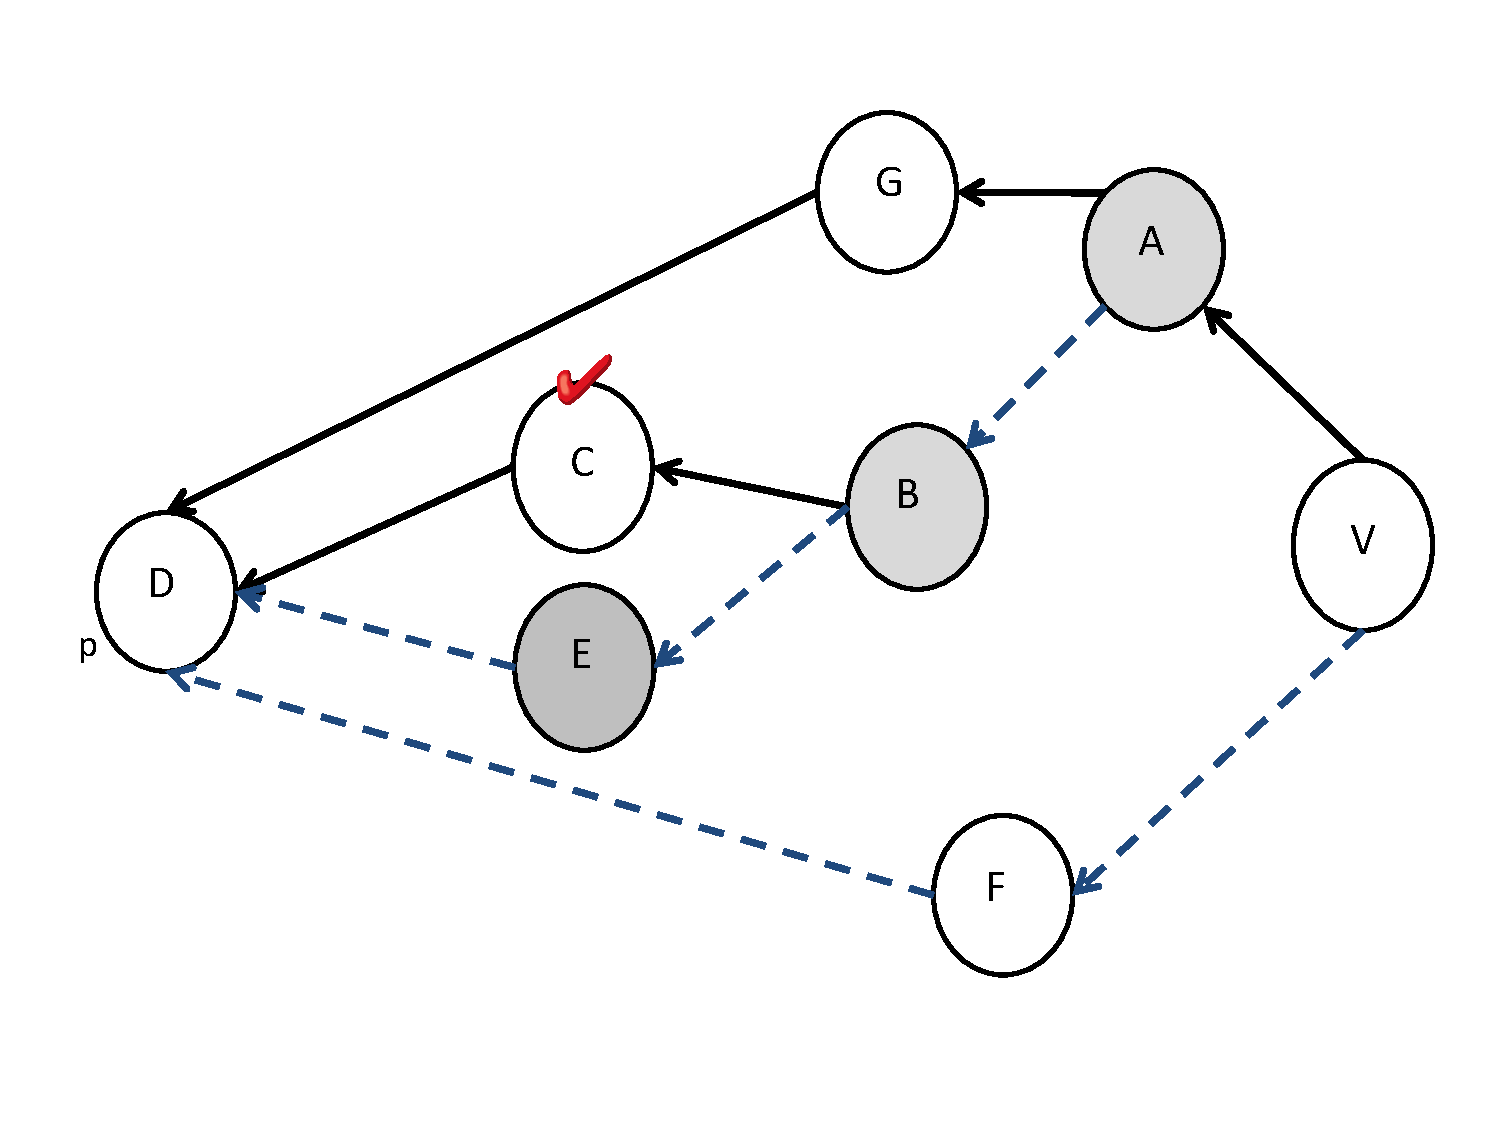
\includegraphics[width=\columnwidth]{figs/general-recur.pdf}
\caption{Hyptothetical topology demonstrating how a routing event 
can induce path changes in a distant part of the topology. 
The ASes shown can be anywhere on the path. \ic{change $D$ for $S$,
G-->D should be dashed. why is E shaded? should C be shaded?}}
\label{fig:recur}
\end{figure}


A generic algorithm for root cause analysis must account for the fact that 
routing changes can take place due to decisions made at a relatively distant AS.
In the case of an induced path change, the origin of the routing instability may not be either
on the old or the new path from the source to destination.
Consider, for example, Figure \ref{fig:recur}, where AS $S$ announces prefix $p$
to the Internet, observed at a vantage point located in AS $V$.
Initial paths are represented by dashed lines and data is forwarded
in the direction of the arrows. Paths after the routing change are represented by
solid lines.  Suppose all path changes
shown are policy compliant. \tbd{DRC: Why would we not otherwise assume this?}
Suppose that $B$, originally using a path
through $E$, switches to the path through $C$ due to a previously unavailable link $B-C$ coming online. 
This new path exported by $B$ is less 
preferable to $A$ than another available path through $G$, causing $A$ to switch 
its paths as well. Finally, $V$ prefers the new path advertised by $A$ to its old
path through $F$. Hence we observe a new path through $A$ and $G$ at $V$ toward prefix $p$. 

In this case, a routing change originating at $C$ has caused three other ASes to change their paths 
in a cascading fashion. This suggests a general recursive algorithm for pinpointing the
root cause of an Internet AS-level path change, a sketch of which is
presented in Figure \ref{fig:gen-algo}. We assume that a path change from the old path
$O(V)$ to the new path $N(V)$ is observed at vantage point $V$. We also
assume that, at any point
in time, only one routing event happens in the topology, where the event could be a 
change in policy, a change in OSPF weights, a link going down, a link coming up, 
or an operator induced change (e.g., manual LocalPref change). 

The algorithm starts at $V$ and each level of recursion
begins at an AS where the old and new paths diverge. For example, in Figure \ref{fig:recur} $V$ is the
vantage point at level 1 since it is where the first path change is observed, $A$
is the vantage point for level 2, and so on. \ic{the problem with
counting towards the origin is that the root cause might be at any
level and ASes that have paths that use the vantage point where the
change was observed might have negative levels.  I suggest we put the root
cause at level 1 (or zero) and then count toward
the observation point.  This is minor, but eases explanation of 
Fig.~\ref{fig:induced}.}  Notice that the recursion halts when it reaches 
the origin of the prefix, i.e., $S$.

\begin{pseudocode}
%\framebox[\columnwidth][l]{
%\parbox{\columnwidth}{
\textbf{RootCause} at AS $V$ \\
\textbf{Given:} $O(V)$ and $N(V)$ toward origin AS $S$ \\
\hrule
\textbf{if} $O(V)$ is the same as $N(V)$: \\ %or current recursion depth is $D$ \\
\hspace*{0.2in} \textbf{return} $\boldsymbol{\emptyset}$ \\
\textbf{for each} AS $A$ in $O(V)$ in order of propagation from $S$: \\
   \hspace*{0.2in} \textbf{if} $A$ has already been visited \textbf{then continue} \\
   \hspace*{0.2in} \textbf{R}$(A) \leftarrow$ \textbf{RootCause} at AS $A$ \\
   \hspace*{0.2in} \textbf{if} \textbf{R}$(A) \ne
\boldsymbol{\emptyset}$ \textbf{then} \textbf{return} \textbf{R}$(A)$:  \\
\textbf{for each} AS $A$ in $N(V)$ in order of propagation from $S$ \\
   \hspace*{0.2in} \textbf{if} $A$ has already been visited \textbf{then continue} \\
   \hspace*{0.2in} \textbf{R}$(A) \leftarrow$ \textbf{RootCause} at AS $A$ \\
   \hspace*{0.2in} \textbf{if} \textbf{R}$(A) \ne
\boldsymbol{\emptyset}$ \textbf{then} \textbf{return} \textbf{R}$(A)$  \\
\textbf{return} $V$

\caption{General recursion-based algorithm for discovering root cause}
\label{fig:gen-algo}
\end{pseudocode}

%There a number of challenges with this general method. 
Given the ability to find paths from the set of ASes discovered in this recursion
at fine-grained intervals, the algorithm
would discover the root cause of a path change. This introduces two key challenges: 

\begin{enumerate} 
\item All ASes discovered need to be monitored
for path changes toward the prefix. This set might be prohibitively large since 
in the worst case the recursion could traverse all \ic{any?} possible policy compliant 
paths from $V$ to $S$. 
\item The path from an arbitrary vantage point needs to measured at fine enough
granularity such that the path is available before and 
after a routing change occurs. 
\end{enumerate}

In the next subsection we address the first challenge, while the second challenge
is addressed in \S \ref{sec:paths}.

\subsection{Bounding the Candidate Set}

To deal with the challenge of monitoring a prohibitively large set of
ASes, we attempt to determine an approximate bound on the candidate set of ASes that 
most likely caused the path change. Our bounding constraints are based on a simple and widely used
model for the BGP decision process~\cite{CaesarR05}. \tbd{DRC: I think we want most of Arvind's original model here.} In short, when multiple
neighbors announce paths toward the same prefix, an AS considers the
economic relationship between neighbors before AS path length.
Typically an AS would prefer paths learned
from customer ASes over those learned from peers and providers \ic{but
this is not all, right? for example, AS $x$ may prefer routes from provider
$p_1$ over routes from provider $p_2$}. If two paths
are equally preferred under this criterion, the path with the shorter AS path
length is picked. Assuming this sequence of decision criteria, we infer a bound
on the candidate set for root cause analysis.
%
\begin{comment}
Feldman et al.~\cite{feldman} constrain this set to include only
those ASes that appear either on the old or the new path. This hypothesis
is based on a limited routing model that assumes that the origin of the
routing change must lie on the 'best' path, which must be either the old
path or the new path. 
\end{comment}

In addition to the notation used above, we use the following notation.
$N(O(V))$ is the set of ASes that appear on the new paths
originating from the ASes in $O(V)$, and $O(N(V))$ is the set of ASes
that appear on the old paths originating from ASes in $N(V)$. 
Note that all ASes in $O(V)$ appear in $N(O(V))$ and that
all ASes in $N(V)$ appear in $O(N(V))$. We claim
that the root AS responsible for a path change is contained in the set 
$\boldsymbol{N(O(S)) \cup O(N(S))}$.

\tbd{DRC: Are we still doing an appendix with the full proof?}
\textbf{Proof Sketch.} We give a sketch of the proof of our assertion
using Figure~\ref{fig:recur}. It is obvious that the root cause might lie on
either the old or the new path, i.e., ASes like $F$ and $A$. ASes in the
set $O(N(V))$, like $B$, can be the root cause as well.
For example, if $B$
is the origin of a link failure and withdraws the path from $A$, $A$ is forced to
switch its path. AS $V$ may then change its route from $F$ to $A$.  
Another example is when $B$ independently switches to a longer path
due to, e.g., a policy change; AS $A$ might not prefer this longer path to another
path available to it that is shorter. The case of $N(O(V))$ is similar.

\tbd{DRC: I think we need to be explicit about what we mean by the additional hops represented by the dots.}
Now we show 
the converse, i.e., that the root cause cannot be ASes like $C$ that are in $N(O(N(V)))$.
\ic{either the following requires some assumptions that we should recall
here; or the example given in Sec. 3.1 cannot happen (in which case we
should show why)}
Assume that
the root cause is $C$ and that $B$ switches to the path through $C$;
suppose further that
$A$ switches to the path through $G$. This implies that $A$'s criterion for path selection
among $G$ and $B$ is AS path length; if it were a favorable business relationship with $B$ then it would have
continued preferring the route through $B$. Shortest path routing implies that
$|A,B\ldots{}E\ldots{}D| \leq |A,G\ldots{}D| \leq |A,B\ldots{}C\dots{}D|$
since $A$ prefers the path through $B$ before the routing event and the
path through $G$ after.
Now, if $V$ switches to the new path through $A$, then
it implies that $V$ is using shortest path routing as well and that
$|V,A,G\dots{}D| \leq |V,F\ldots{}D| \leq |V,A,B\ldots{}E\ldots{}D|$
since $V$ prefers the path through $F$ before the routing event and the
path through $A$ after.
This, however, contradicts the earlier result from $A$
that $|A,B\ldots{}$ $\ldots{}E\ldots{}D| \leq |A,G\ldots{}D|$. Hence, $C$ cannot be
the root cause.  \tbd{DRC: Is there a similar argument for $O(N(O(V)))$? If so, we should say so.}Therefore the root cause is constrained to the set $N(O(S)) \cup O(N(S))$.

Now that we have bounded the set of candidate ASes for root cause, we describe
the different approaches to identify the set of ASes in this set.

\subsection{Computing the Candidate Set}
\label{sec:paths}

\begin{enumerate}

\item \textbf{Constant Monitoring of Prefixes for Path Changes.} The first
way to identify the ASes in the candidate set is to continously monitor
and store paths toward a prefix through a distributed set of vantage points. For a 
given vantage point $V$, paths to the prefix-originating $D$ are measured 
periodically. Whenever a path change is observed in the wild, in addition 
to accounting for the ASes that appear in $O(V)$ and $N(S)$, paths from
other vantage points are queried so that other ASes in $N(O(V))$
and $O(N(V))$ are discovered. This is shown in Figure \ref{fig:computeset}. 
In practice this monitoring system would be similar to iPlane \cite{iplane} and 
the UCLA Internet Topology Collection project \cite{ucla-topology}.

\begin{figure}[!htbp]
\centering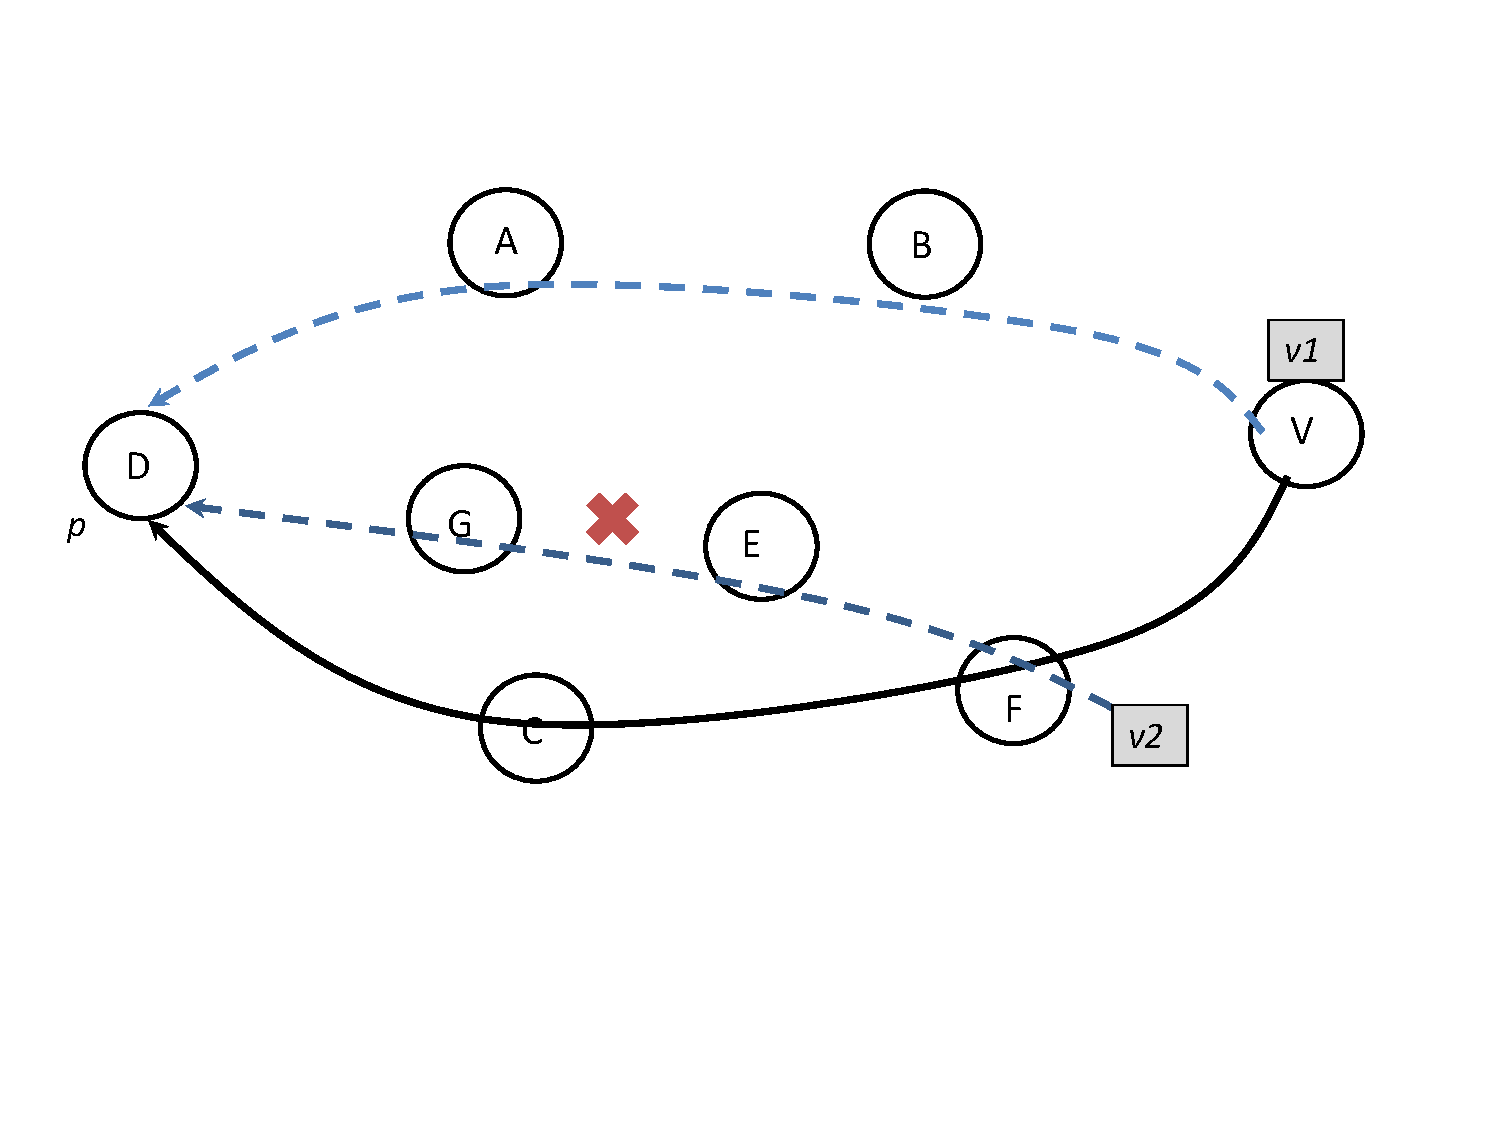
\includegraphics[width=\columnwidth]{figs/computeset.pdf}
\caption{Identifying ASes in the root cause candidate set. When a path change
is observed at vanatge point \emph{v1} (dashed to solid line), 
current and historical paths are queried from other vantage 
points such as \emph{v2} that might have passed through ASes in the old
and new paths. For example, the path from \emph{v2} passes through $F$, an AS
on the new path from $V$ to $D$, allowing us to find out ASes on the
older path from $F$.}
\label{fig:computeset}
\end{figure}

Waiting for actual path changes to take place in the wild will
likely be inefficient as well as insufficient for the purposes of identifying
all the ASes in the candidate set for any number of vantage points. 

\item \textbf{Path Prediction.} Another approach for 
computing the candidate set is to predict all 
policy compliant paths from a vantage AS $V$ to destination $D$
in an offline fashion. For example, \emph{iPlane} \cite{iplane} uses 
traceroute data to do so. The disadvantage of this approach 
is that it may generate an extremely large set of policy compliant 
paths that are unlikely to ever be used. In Section~\ref{sec:ases_to_monitor}, we show that such an approach could require monitoring many paths. Because our goal is to 
produce a reasonably bounded set of paths to monitor, this approach 
is impractical.

\item \textbf{Revealing Alternative Paths via BGP Announcements.} 

The third technique for identifying candidate ASes is a middle ground between
passively waiting for path changes to happen in the wild and predicting all 
valley-free paths offline (some of which might not actually be used). It uses
BGP loop prevention (commonly referred to as 'poisoning' \cite{optometry,lorenzo-thesis}) 
to explore less preferred paths from an AS toward a prefix we control.
Specifically, when we target AS $X$ for exploration we include its ASN in our 
announcements. This causes AS $X$ to reject the route due to loop detection; 
this in turn forces the ASes 
that previously routed through $X$ to find alternate routes toward the destination.
Once poisoning has generated a path change, paths from a distributed set of
vantage points are queried to find ASes in the old and new paths from ASes $O(V)$ 
and $N(V)$. In Figure \ref{fig:computeset}, poisoning $E$ simulates a link-down 
event for $G-E$ as $E$ withdraws all announcements for prefix $p$
from its neighbors, causing $F$ to choose the path through $C$.

\end{enumerate}


